\documentclass[sigconf]{acmart}


%!TEX root = report.tex
% Packages
\usepackage{url}
%\usepackage[pdfpagelabels=false]{hyperref}
\usepackage{graphicx}
\usepackage{multirow}
% \let\proof\relax
% \let\endproof\relax
\usepackage{amssymb}
\usepackage{amsmath}
\usepackage{centernot}
\usepackage{amsthm}
\usepackage{algorithm}
\usepackage[noend]{algpseudocode}
\usepackage{enumerate}
% \usepackage{colortbl}
\usepackage{balance}
\usepackage{enumitem}
% \usepackage[dvipsnames]{xcolor}
\usepackage{rotating}
\usepackage{tikz}
\usepackage{enumitem}
\usepackage{balance}
\usepackage{soul}
\usepackage{subcaption}
\usepackage[framemethod=tikz]{mdframed}
\usepackage{xspace}
\usepackage{makecell}
\usepackage{hyphenat} % handle hyphenations with \hyp{}
\usepackage{pifont} % for table marks
\usepackage{soul}
\usepackage{mathtools}
\usepackage{float}

\usetikzlibrary{decorations.markings}
%%
%% The next line says how the "vertex" style of nodes should look: drawn as small circles.


\hypersetup{
%    bookmarks=true,         % show bookmarks bar?
    unicode=false,          % non-Latin characters in Acrobats bookmarks
    pdftoolbar=true,        % show Acrobats toolbar?
    pdfmenubar=true,        % show Acrobats menu?
    pdffitwindow=false,     % window fit to page when opened
    pdfstartview={FitH},    % fits the width of the page to the window
    pdftitle={My title},    % title
    pdfauthor={Author},     % author
    pdfsubject={Subject},   % subject of the document
    pdfcreator={Creator},   % creator of the document
    pdfproducer={Producer}, % producer of the document
    pdfnewwindow=true,      % links in new window
    colorlinks=true,       % false: boxed links; true: colored links
    linkcolor=black,          % color of internal links
    citecolor=black,        % color of links to bibliography
    filecolor=black,      % color of file links
    urlcolor=black,           % color of external links
}



\newcommand*{\graphpair}[2]{\langle #1, #2 \rangle}
\newcommand*{\tuple}[1]{(#1_1, ..., #1_n)}
\newcommand*{\range}[3]{#1 = #2 ... #3}
\newcommand*{\pair}[2]{(#1,#2)}
\newcommand*{\triple}[3]{(#1,#2,#3)}
\newcommand*{\edge}[4]{#1 \overset{#3}{#4} #2}
\newcommand*{\uedge}[2]{\edge{#1}{#2}{}{--}}
\newcommand*{\dedge}[2]{\edge{#1}{#2}{}{\rightarrow}}
\newcommand*{\luedge}[3]{\edge{#1}{#2}{#3}{--}}
\newcommand*{\ldedge}[3]{\edge{#1}{#2}{#3}{\rightarrow}}
\newcommand*{\expgname}[1]{#1^+}
\newcommand*{\expgraph}[3]{\expgname{#1}:\graphpair{#2^+}{#3^+}}


%Paper macros

\setcounter{secnumdepth}{5}

%Algorithmic macros
\renewcommand{\algorithmicrequire}{\textbf{Input:}}
\renewcommand{\algorithmicensure}{\textbf{Output:}}
\renewcommand{\algorithmicforall}{\textbf{for each}}
\algdef{SE}[DOWHILE]{Do}{DoWhile}{\algorithmicdo}[1]{\algorithmicwhile\ #1}%

%Complexity macros
\newcommand*{\NP}{$\mathbf{NP}$}
\newcommand*{\NPhard}{$\mathbf{NP}$-hard}
\newcommand*{\NPcomplete}{$\mathbf{NP}$-complete}
\newcommand*{\SPcomplete}{$\mathbf{\#P}$-complete}
\newcommand*{\SPhard}{$\mathbf{\#P}$-hard}
\newcommand*{\bigO}{\mathcal{O}}

% Paragraphs
\newcommand{\spara}[1]{\smallskip\noindent{\bf #1}}
\newcommand{\mpara}[1]{\medskip\noindent{\bf #1}}
\newcommand{\para}[1]{\noindent{\bf #1}}

\newcommand{\blackBox}{$\blacksquare$}
\newcommand\todo[1]{\textbf{\textcolor{red}{#1}}}



\setcopyright{none}



%DO NOT CHANGE THE INFO BELOW
\acmDOI{}
\acmConference[GM 2017]{Graph Mining Project}{February, 18 -- 2018}{Potsdam} 
\acmYear{2018}
\copyrightyear{2018}



\title{Finding Hidden Communities in HackerNews}
\subtitle{Graph Mining - WS 2017/18 - Project Report}

%\institute{}

% \date{Due date: February 18, 2017}

\author{Willi Gierke}

\author{Fabian Paul}

\renewcommand{\shortauthors}{}


\begin{document}


% GENERAL rules: 
% Substitute the content in [] brackets with the actual 
% Do not change the other information in the template, if you want to add some package, modify the file macros.tex
% Preferably include pictures with high resolution or vectorial pictures (even better) in pdf.



% - Summary of the project
\begin{abstract}
% Brief description of the project: used network and the performed analysis. 
HackerNews\footnote{\url{https://news.ycombinator.com/}} is a news site focusing on entrepreneurship and computer science.
Users are able to post stories or comment on these.
Unlike social networks, users can not add friends or join groups.
We were interested in whether it is still possible to find communities just based on the information which stories users commented.
\end{abstract}

\maketitle



\section{Data Preparation}
% Report the main characteristics of the dataset (or datasets) that you used. This includes: number of nodes, number of edges, whether directed/undirected graph, static/dynamic graph, number of node/edge labels (if labeled), presence of ground truth (e.g., communities, classes to learn ...), degree distribution.

% [Optionally] You can report more fine grained information, such as the number of connected components in the graph, the size of the largest/smallest connected component, the diameter, the number of triangles.


The dataset we used was published on reddit\footnote{\url{https://www.reddit.com/r/datasets/comments/6v685o/complete_hacker_news_ycombinator_data_dump/}} and contains a complete dump of all stories and comments of HackerNews between its launch in 2006 and July 2017 in CSV format.
The dataset contains 9.9M comments and 2.1M stories posted by 400k users. 

Due to the amount of data, we could not clean and preprocess all CSV files every time we wanted to build a graph. We decided to read all the files once and store them in a SQLite\footnote{\url{https://www.sqlite.org/}} database on disk. With this approach, we also avoided mixed column types because we specified our types first in a pandas Dataframe and saved it as CSV file afterwards.
Unfortunately, not all of the CSV files shared the same schema so we had to select our important columns first before inserting them into the database. 

It was important for us to select a subset of comments because of the increasing complexity of building the graph and computation time of all used algorithms. Especially the SQL projection to select just the columns we needed to reduce the amount of main memory we were supposed to allocate drastically.



\section{Graph Building} \label{graph_building}
% \begin{itemize}
%   \item Report all the preprocessing steps to obtain the final network. How do you store the data (graph database, main memory, disk)? In which format? Did you have to remove some information in order to clean the data? 
%   \item Report also preliminary analyses and insights about the data. 
%   \item At least one picture with the graph visualized \textbf{must} be included. Use a software for visualization, like Gephi\footnote{\url{https://gephi.org/}}
% \end{itemize}

% \begin{figure}[htb]
% 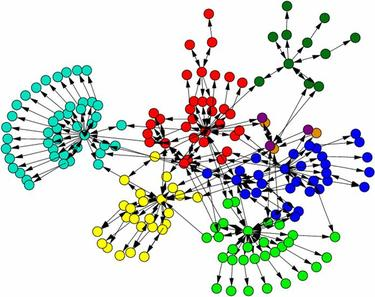
\includegraphics[width=\linewidth]{images/network.jpg}
% \caption{Our network.}
% \label{fig:network}
% \end{figure}



% \begin{itemize}
%   \item reference pandas
%   \item reference igraph
%   \item igraph object in main-memory, GraphML format when persisted
%   \item we omit features like time, scores etc.
%   \item insert igraph picture here
%   \item no labels
%   \item number of connected components
% \end{itemize}

We have built a tool to quickly extract all the needed information from the database and build the graph based on it. It is possible to build graphs on any arbitrary subset of the data. 
Our graph building approach is iterating over the extracted data, looking for every comment for its parent comment or story. Since we have to traverse the whole subset in every line, the resulting runtime is in $O(n^{2})$ where $n$ is the number of rows.

In the end, each node represents a user.
An edge between two nodes is drawn if they have commented the same story.
In the case of users sharing multiple commented stories we just draw one edge to avoid duplicates.
The graph, therefore, is undirected and unweighted.
In the following, we will use two different graphs based on different subsets.


% It is further a static graph since no nodes or edges are added or removed once the graph has been created. \todo{check whether that is correct}
% We pruned the graph using \todo{X} to only contain \todo{Y nodes or Z edges}.
% Unfortunately, there is no ground truth available we could refer to for comparing found communities.
% The degree distribution of the graph can be seen in Figure \todo{X}.
% Its diameter is \todo{X} and there are \todo{X} triangles present.


\section{Description of the algorithms}
% Briefly describe in your own words the algorithm or the algorithm(s) you used in terms of input and output, which kind of network it applies to, and what is the main idea behind it (three sentences). Reference the algorithm (e.g.,\cite{zhao2007graph})

The following section gives a brief overview what kind of community detection algorithms we used.
We will also give a short explanation why we decided to use these algorithms and how they work. 
Allowing a good comparison between those we chose three algorithms which try to optimize the modularity while applying their procedures. Our choices were also strongly influenced by the implementation given by the igraph\footnote{\url{http://igraph.org/}} framework because it is one of the few frameworks which offers all implementation in fast C code. Fortunately, we could use the provided python bindings to keep our analysis simpler. Specifically, we looked for algorithms which offer quick results and we do not have to wait multiple hours to run the community detection algorithms on our graphs.

\subsection{Fast Greedy} \label{fast_greedy}

The first algorithm we selected was developed by Clauset et al. \cite{clauset2004finding} in 2004. This algorithm was specially developed for the physics community due to its need for analyzing big networks. It provides a run time of $O(m*d* log(n))$ hereby is $m$ the number of edges, $n$ the nodes and $d$ is the depth of the dendrogram describing the community structure. Clauset et al. took the assumption that many real-world graphs are sparse and hierarchical therefore $m \sim n$ and $d \sim log(n)$ which leads to an almost linear run time.

In summary, the algorithm tries to assign nodes to certain communities maximizing the modularity greedily. If there are no improvements to the modularity possible, which can be done through a node reassignment, the algorithm terminates.



\subsection{Leading Eigenvector}

The idea of the Leading Eigenvector\cite{newman2006finding} approach is to split the graph successively into densely connected communities based on the eigenvector of the biggest eigenvalue of the modularity matrix.
The modularity matrix is defined as the difference between the symmetric adjacency matrix of the graph and $P$.
$P[i, j]$ contains the probability that node $i$ shares an edge with node $j$.
Obviously, $P$ is symmetric as well.
After calculating the eigenvector of the biggest eigenvalue of the modularity matrix, the graph is split based on the sign of the corresponding node in the eigenvector.
If all entries in the eigenvector share the same sign, the network is assumed to have no underlying community structure.
As described by Newman\cite{newman2006finding}, since the proposed method runs in polynomial time and the problem of modularity optimization is NP-hard, one can be certain that the algorithm does not yield the best result in all cases.
% As part of our investigations, we neither were able to notice significant performance improvements nor have we perceived better modularity results. A reason might be that the computed graphs are degenerate which leads to unstable solutions of the eigenvector solver.


\subsection{Louvain}

In comparison to the first described algorithm, this one tries to optimize the modularity similarly.
The algorithm got its name from its authors Blondel et al. \cite{blondel2008fast} because the main part of the work was done within the Universit\'e catholique de Louvain.
Unfortunately, there is no existing proof for the runtime but it is presumably considered as $O(nlog(n))$.

Each vertex will be assigned to a community initially rather than a node as described in Subsection \ref{fast_greedy}.
Iteratively, the algorithm moves vertices between communities to optimize the modularity every round.
After every round, all found communities are shrunk to a single vertex and the process continues until the modularity of the graph cannot be further optimized by moving vertices. 


\section{Network analysis}
% In this section, explain thoroughly the steps of the analysis you performed and give a motivation for such an analysis (e.g. discovering the most influential node, finding interesting patterns, analyzing communities). Elaborate on why you find it challenging and useful. Report possible applications.  

Even though there is not a direct relation between users on HackerNews, we wanted to see if users can be grouped by their opinions.
Hence we might find them commenting on the same stories.

First, we tried building the full graph on all years of posts. Unfortunately, we quickly discovered that building the graph would take a long time and a lot of RAM, more than a normal laptop could provide. With the method described in Section \ref{graph_building} we started using specific user groups.
Figure \ref{fig:user_hist} indicates that the majority of users is not commenting very often rather just having a few comments at all.

\begin{figure}[h]
    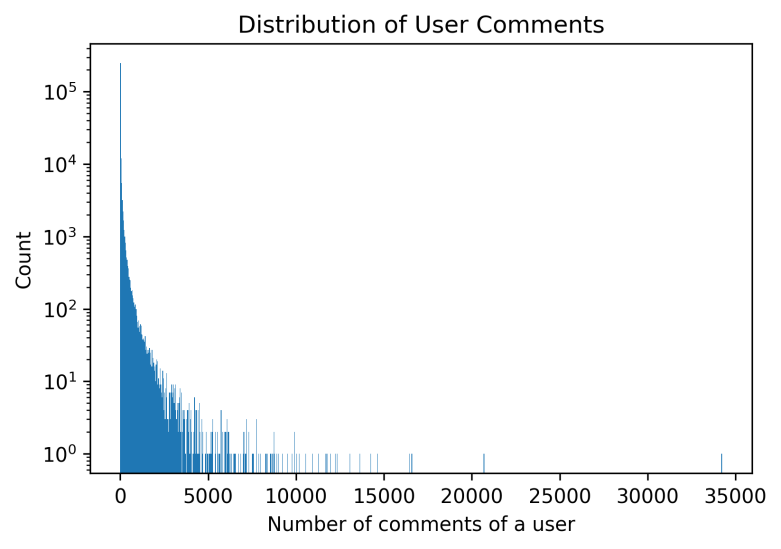
\includegraphics[width=\textwidth / 2]{images/user_hist.png}
    \caption{User comments histogramm extracted from the full dataset}
    \label{fig:user_hist}
\end{figure}

In the following section, we will mainly work with two subsets of user groups and its resulting graphs.
Table \ref{graph_sum} should give a short overview what kind of graphs we are analyzing.

\begin{table}[H]
\centering
\begin{tabular}{|l|l|l|}
\hline
               & Middle 10k & Top 10k \\ \hline
Edge Count     & 38914      & 170204   \\ \hline
Average Degree & 5.959      & 17.348  \\ \hline
Diameter       & 11         & 8       \\ \hline
\end{tabular}
\caption{Graph summary}
\label{graph_sum}
\end{table}

\subsection{Top 10k Users}

With this knowledge, we created our first graph by selecting the top 10000 most commenting users. We still noticed that the graph was growing too fast especially the number of edges when working on the full dataset.
We filtered the underlying data by only considering comments posted in January 2017.
Our assumption was to find good communities with a high modularity due to the high number of comments. 
This might have been a misconception which can be seen in Figure \ref{fig:top_10k} 

\begin{figure}[H]
    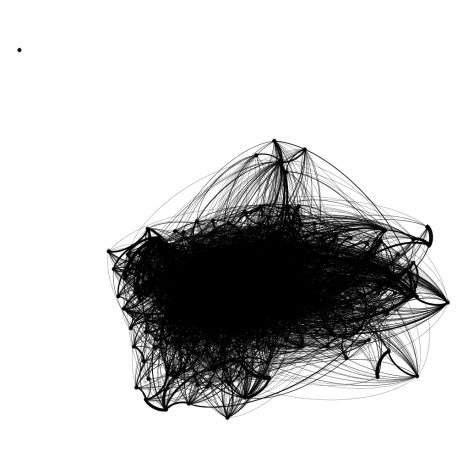
\includegraphics[width=\textwidth / 2]{images/top_10k.png}
    \caption{Graph subsampled with the top 10k users and January 2017}
    \label{fig:top_10k}
\end{figure}

The resulting graph is highly connected and does not imply any communities while looking at it. That is why we assumed that the top 10000 users are not very representative for the all users on HackerNews. 

\subsection{Middle 10k Users}

Our next idea was building the graph with a user group somewhere in the middle of the histogram in Figure \ref{fig:user_hist}.
This might lead to a better user distribution based on their opinions since we have limited the number of overall comments.
The graph was built with the first 10000 users ordered by the comment count per user having more than 50 comments. 

\begin{table}[h]
\centering
\begin{tabular}{l|l|l}
Algorithm           & Time & Modularity \\ \hline
Fast Greedy         & 1s   & 0.46       \\ \hline
Louvain             & 1.1s & 0.46       \\ \hline
Leading Eigenvector & 3.8s & 0.41      
\end{tabular}
\caption{Community detection performance on full graph}
\label{full_comm}
\end{table}

In Table \ref{full_comm} one can see that all community algorithms find significant community structures due to $0.4 < modularity < 0.7$ which usually indicates how good the detection algorithm performs.
Although the first two algorithms running almost the same time and performing equally, the Leading Eigenvector algorithm is more than three times slower and also performing worse.
In general, we would have expected a better result from the Leading Eigenvector algorithm since the approach itself tries to directly optimize the community splits depending on the modularity matrix and not on moving edges or nodes.
A reason might be that the computed graph is degenerated which leads to an unstable solution of the eigenvector solver which is needed for the algorithm.

To further improve the modularity of our partitions we investigated in removing very tiny communities which are just increasing the complexity.
Therefore we built the biconnected components of the graph as shown in Figure \ref{fig:biconnected}.

\begin{figure}[h]
    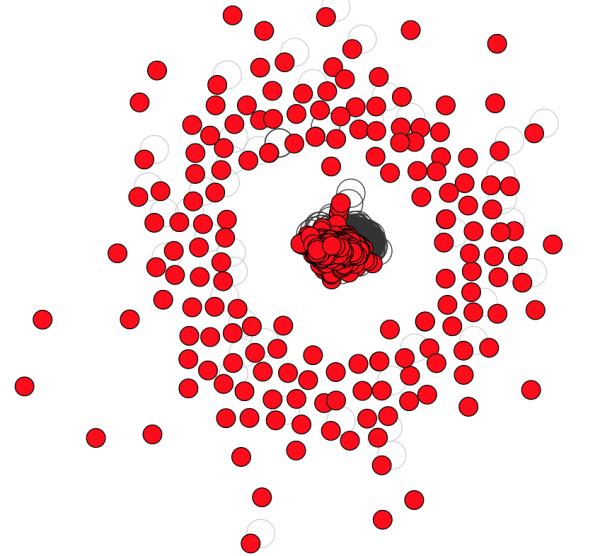
\includegraphics[width=\textwidth / 2]{images/biconnected.png}
    \caption{Biconnected components of full graph}
    \label{fig:biconnected}
\end{figure}

The newly formed graph has a node for every detected component and an edge if the components are connected.
Hereby we are not showing the articulation nodes which would not belong to one component only to get a better overview of the overall structure.
Henceforth we will describe the inner components as \textit{Core}. 

Following the idea mentioned before we are just concentrating on the \textit{Core} and removing the surrounding components to build a new graph.
The reduced graph has roughly 700 nodes and edges less than the one looked at before.

\begin{table}[h]
\centering
\begin{tabular}{l|l|l}
Algorithm           & Time & Modularity \\ \hline
Fast Greedy         & 408ms   & 0.45       \\ \hline
Louvain             & 780ms & 0.45     \\ \hline
Leading Eigenvector & 2.95s & 0.37      
\end{tabular}
\caption{Community detection performance on core graph}
\label{core_comm}
\end{table}

In comparison to the results on the full graph, nothing significant has changed.
All algorithms are faster but slightly less accurate.
This means even with the removal of small components the algorithms cannot find better community structures.
Nevertheless, the number of communities was drastically reduced from 204 to 38 in the \textit{Core}.

Given a more structured view seen in Figure \ref{fig:comm_graph} it is noticeable that the formed communities closely relate to the found biconnected components shown in Figure \ref{fig:biconnected}. 

\begin{figure}[h]
    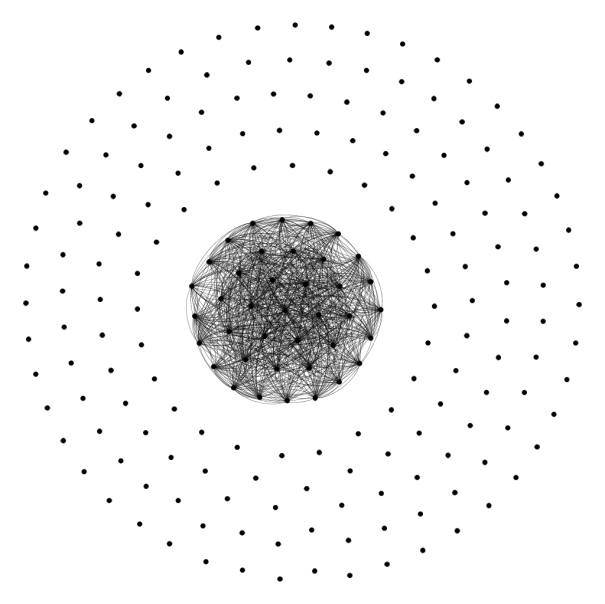
\includegraphics[width=\textwidth / 2]{images/comm_graph.png}
    \caption{Extracted communities with the Louvain algorithm}
    \label{fig:comm_graph}
\end{figure}

One reason for the dense core could be that a usual user of HackerNews is commenting a lot of stories but without a meaningful or predictable background.

% \begin{itemize}
%   \item analyze communities in order to find popular topics people talk about without having friendship relations, groups, channels etc.
% \end{itemize}

% \subsection{Qualitative Results}
% % Comment the results of the analysis. You should also mention all the relevant details of your analysis, for instance specific values for parameters you used. It is preferable that you show some graphics and present some examples. If you use a visualization method to depict the nodes of the graph, make sure that you can explain at least a part of the network in the plot. 

% % For instance for node classification, show some of the classified vertices. If you have a ground truth, compare it to your results. You can also show a use case by running the algorithm on a smaller network (like the Star Wars network) and show what you find. 

% % For a graph query, show how the algorithm behaves with particular patterns (stars, triangles, cores ...).  Is the algorithm producing useful and interpretable results? Are the results unexpected or is it something you can find by yourself? Is there some anomaly?

% \begin{itemize}
%   \item a lot bi-components: represent people that prefer to comment only on specific topics only (comparison with DL/Trump graph)
%   \item dense core: people seem to comment randomly on stories. They tend to not give technical feedback or evaluations but comment on the stories in a more abstract fashion or make jokes
% \end{itemize}

% \subsection{Time and Scalability}
% Evaluate the used method regarding its run time and scalability. Report the time you need to preprocess  the data (if there is such a phase, like an index construction) and to produce the results. On the same network and algorithm, consider incremental graph sizes (e.g. 10\% of the network, 30\%, etc.). 

% \smallskip
% \noindent Alternatively, generate some random network with \url{http://www.cse.ust.hk/graphgen/} or any other graph generator and compare the results of the algorithm between the two graphs (the original one and the random one). Are there any important differences in the outcome? Specify the parameters of the graph generator of choice. 

% \begin{itemize}
%   \item building graph takes 15 minutes due to $N^{2}$ manner of graph building and slow Python bindings (probably?)
%   \item time of algos from table
% \end{itemize}


% \subsection{[Optional] Memory usage}
% % Report how much memory is consumed by the algorithm. 

% \begin{itemize}
%   \item use htop :-)
% \end{itemize}


\section{Limitations and interesting findings}
% Did you notice any limitation in the approach? Does it work as expected regarding the quality of the results? In terms of performance, is it too slow when the network is too big? Is it domain dependent or applicable to various types of graphs? To which kind of users are the results of the analysis useful? Describe what you have learned and propose ideas on how the analysis could improved. 

When analyzing the underlying dataset, we noted several power law relationships.
As an example, we already presented the number of user comments in Figure \ref{fig:user_hist}.
The number of comments and the scores of a story also follow this distribution which peaks at zero.
Since this expresses a high skewness of the underlying data, the results of the community detection algorithms might be improved if one filters the considered comments more extensively.
This could, for example, be done by building the graph based on comments that belong to stories with a score above a certain threshold.
An other possibility would be to only consider stories that are connected with a minimum number of comments to better select popular stories.

An other limitation is that the communities are barely interpretable and there is no ground truth to compare the results with.
To overcome these issues, one could apply topic modeling based on the comments of the users.
This way, one can not only find common topics users talk about but by aggregating the comments of a user one can find his "favorite topic".
This way, each user can be labeled with his favorite topic and the found communities can be compared with the topic labels using e.g. mutual information\cite{cover1991information}.
The idea behind this approach is that users who comment the same stories are expected to also comment on the same topics.

In our presented approach we assumed the graph to be unweighted.
However, it might make sense to consider weighted edges since initially we deduplicated edges which may be used for weighting.

\section*{Acknowledgement}
We would like to thank Anton Tsitsulin for providing the data which we used to build the graphs.

% - Bibliography
\bibliographystyle{ACM-Reference-Format}
\bibliography{bibliography}  

\end{document}
